\section{Auswertung}
\label{sec:Auswertung}
\subsection{Messdaten}
Im Folgenden sind die nach Kapitel \ref{sec:Durchführung} aufgenommenen Messdaten tabellarisch aufgelistet.

\begin{table}[H]
    \centering
        \caption{Abmessungen und Gewicht der Proben, wobei $d$ bei Stab 1 und 2 die Dicke und bei Stab 3 den Durchmesser beschreibt.}
        \label{tab:abmessungen}
        \sisetup{table-format=3.1}
        \begin{tabular}{S S[table-format=1.1] S[table-format=2.1] S}
          \toprule
          {Probe} & {$d/\;\si{\centi\metre}$} & {$L /\;\si{\centi\metre}$} & {$m /\;\si{\gram}$}\\
          \midrule
          $\text{Stab 1}$ & 1.2 & 59.3 & 163.1\\
          $\text{Stab 2}$ & 1.1 & 59.3 & 454.6\\
          $\text{Stab 3}$ & 1.0 & 60.2 & 394.1\\
          \bottomrule
       \end{tabular}
    \end{table}

\begin{table}[H]
    \centering
        \caption{Messdaten bei einseitiger Einspannung.}
        \label{tab:einseitig}
        \sisetup{table-format=1.3}
        \begin{tabular}{S[table-format=2.0] S S S}
          \toprule
          &
          \multicolumn{1}{c}{$m_1=\SI{800}{\gram}$} &
          \multicolumn{1}{c}{$m_2=\SI{1250}{\gram}$} &
          \multicolumn{1}{c}{$m_3=\SI{550}{\gram}$} \\
          %\cmidrule(lr){2}\cmidrule(lr){3}\cmidrule(lr){4}
          {$x/\;\si{\centi\metre}$} & {$D_1/\;\si{\milli\metre}$} & {$D_2/\;\si{\milli\metre}$} & {$D_3/\;\si{\milli\metre}$} \\
          \midrule
          5  & 0.099 & 0.050 & 0.085 \\
          10 & 0.360 & 0.180 & 0.317 \\
          15 & 0.781 & 0.400 & 0.730 \\
          20 & 1.321 & 0.799 & 1.210 \\
          25 & 2.152 & 1.100 & 1.900 \\
          30 & 2.860 & 1.525 & 2.600 \\
          35 & 3.350 & 1.900 & 3.280 \\
          40 & 4.155 & 2.333 & 4.145 \\
          45 & 5.030 & 2.805 & 4.875 \\
          50 & 5.820 & 3.300 & 5.530 \\
          \bottomrule
       \end{tabular}
    \end{table}

\begin{table}[H]
    \centering
        \caption{Messdaten bei zweiseitiger Einspannung.}
        \label{tab:zweiseitig}
        \sisetup{table-format=2.3}
        \begin{tabular}{S S}
          \toprule
          &
          \multicolumn{1}{c}{$m_3=\SI{1550}{\gram}$} \\
          %\cmidrule(lr){2}
          {$ x/\;\si{\centi\metre}$} & {$D_3/\;\si{\milli\metre}$} \\
          \midrule
          5  & 0.045 \\
          10 & 0.150 \\
          15 & 0.295 \\
          20 & 0.420 \\
          25 & 0.510 \\
          30 & 0.570 \\
          35 & 0.515 \\
          40 & 0.455 \\
          45 & 0.330 \\
          50 & 0.175 \\
          55 & 0.000 \\
          \bottomrule
       \end{tabular}
    \end{table}

\subsection{Bragg Bedinugung}
\label{sec:brag}
Nach der Bragg'schen Bedingung \eqref{eqn:bragg} tritt das Intensitätsmaximum bei dem Glanzwinkel $\theta_{glanz}=\SI{28}{\degree}$ auf.
In Abbildung \ref{fig:plot1} sind die Messdaten mittels \textit{matplotlib} \cite{matplotlib} graphisch dargestellt. Das Maximum befindet
sich bei $\theta=\SI{28.2}{\degree}$. Die totale Abweichung zu dem Theoriewert beträgt somit $\Delta\theta_{glanz}=\SI{0.2}{\degree}$,
was einer prozentualen Abweichung von $p=\SI{0.71}{\percent}$ entspricht.
\begin{figure}[H]
    \centering
    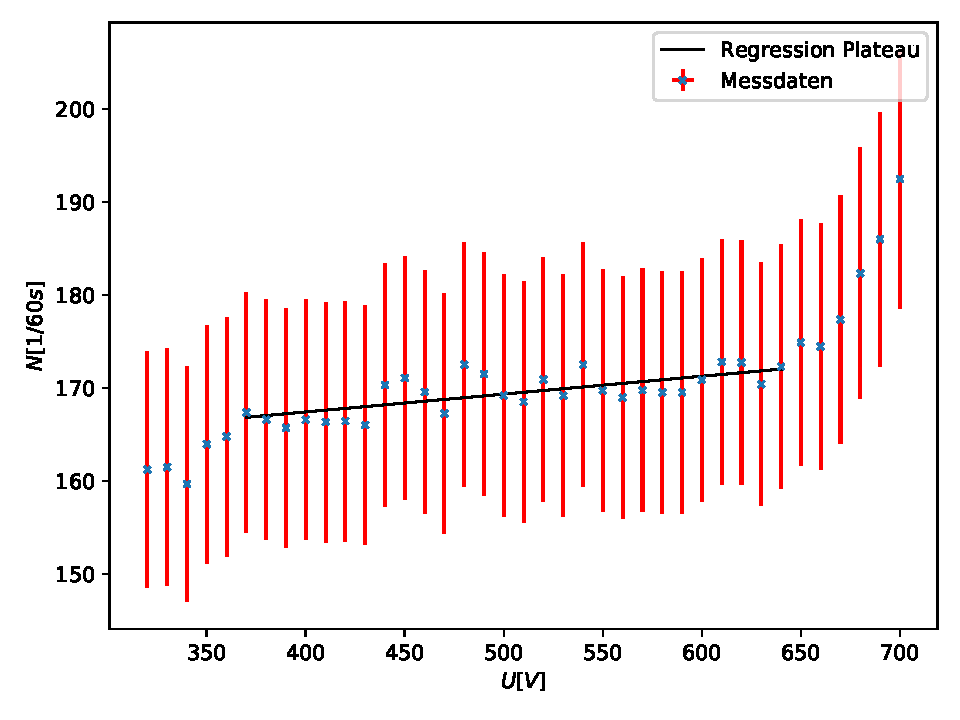
\includegraphics[width=\textwidth]{build/plot1.pdf}
    \caption{Zählrate $N$ in Abhängigkeit vom Winkel $\theta$.}
    \label{fig:plot1}
\end{figure}

\subsection{Emissionspektrum}
\label{sec:emission}
Das nach Kapitel \ref{sec:Durchführung} gemessene Emissionsspektrum wurde in Abbildung \ref{fig:plot2}
als ($\theta-N$)-Diagramm  dargestellt. Dabei sind Bremsberg und die Spektrallinien $K_{\alpha}$ und
$K_{\beta}$ des Kupfers markiert. Die Punkte der jeweiligen Extrema sind in Tabelle \ref{tab:emission} dargestellt und in Abbildung
\ref{fig:plot1} rot unterlegt. Zudem sind in grün die Halbwertsbreiten $\Delta\theta$ der $K_\alpha$ und $K_\beta$-Kante eingezeichnet.
Auch diese finden sich in Tabelle \ref{tab:emission}
\begin{figure}[H]
    \centering
    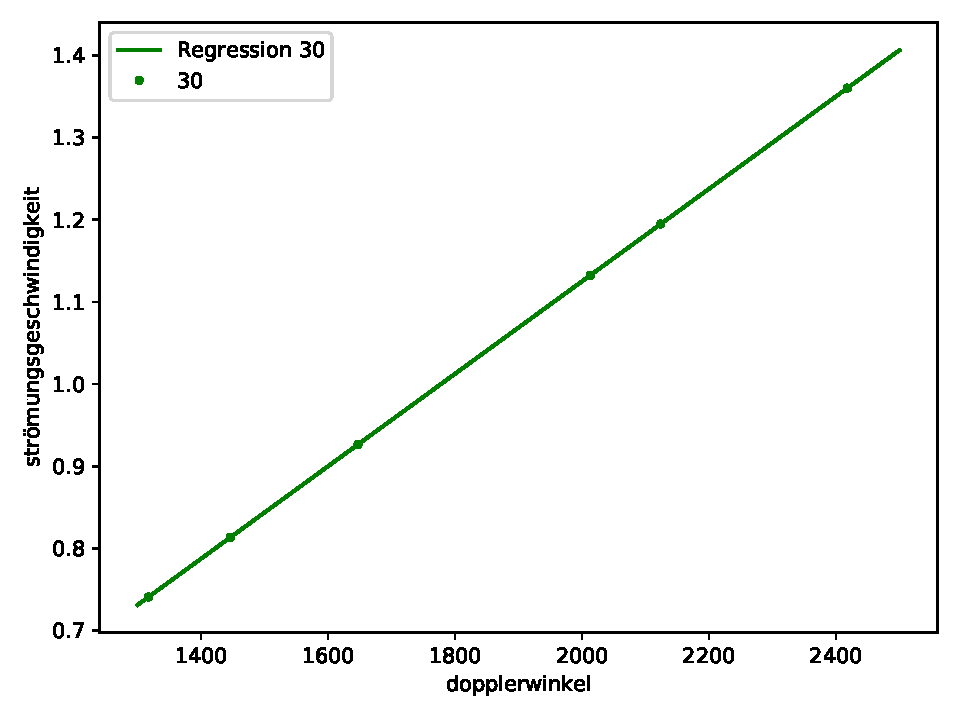
\includegraphics[scale = 1.0]{build/plot2.pdf}
    \caption{($\theta-N$)-Darstellung des Emissionsspektrums.}
    \label{fig:plot2}
\end{figure}
\begin{table}[H]
    \centering
        \caption{Extrema des Emissionsspektrums}
        \label{tab:emission}
        \sisetup{table-format=4.1}
        \begin{tabular}{S S[table-format=2.1] S[table-format=1.3] S}
          \toprule
          {Extremum} & {$\theta [°]$} & {$\Delta\theta$} & {$N [\si{\per\second}]$} \\
          \midrule
          {Bremsberg }   & 11.1 &        &  420.0  \\
          {$K_{\beta} $} & 20.2 &  0.476  & 1599.0\\
          {$K_{\alpha}$} & 22.5 &  0.490  & 5050.0\\
          \bottomrule
        \end{tabular}
      \end{table}
\noindent
Sowohl die Maxima als auch die Halbwertsbreiten wurden dabei mittels \textit{scipy} \cite{scipy} bestimmt.
\\\noindent
Für die Spektrallinien wird nun die Wellenlänge $\lambda$ mittels Gleichung \eqref{eqn:(3)} berechnet und mit dem Zusammenhang
\eqref{eqn:E=hc/lambda} als Energie $E$ angegeben. Die Ergebnisse finden sich in Tabelle \ref{tab:energie}.
\begin{table}[H]
    \centering
        \caption{Photonenenergie bei $K_{\alpha}$ und $K_{\beta}$}
        \label{tab:energie}
        \sisetup{table-format=1.4}
        \begin{tabular}{S S S S}
          \toprule
          {Spektrallinie} & {$E [\si{\kilo\electronvolt}]$} & {Literatur \cite{AP03} $[\si{\kilo\electronvolt}]$} & {p [\%]}\\
          \midrule
          {$K_{\alpha}$} & 8.044 & 8.048 & 0.047 \\
          {$K_{\beta} $} & 8.915 & 8.907 & 0.091 \\
          \bottomrule
        \end{tabular}
      \end{table}
Dabei beträgt die Energiedifferenz über die Halbwertsbreite
\begin{align*}
    \Delta E_{K_\beta}  &= \SI{0.199}{\kilo\electronvolt}\\
    \Delta E_{K_\alpha} &= \SI{0.164}{\kilo\electronvolt}   .
\end{align*}
Die Berechnung des Auflösevermögens $A=E/\Delta E$ ergibt
\begin{align*}
    A_{K_\beta}  &= \num{44.85}\\
    A_{K_\alpha} &= \num{48.92} .
\end{align*}

Aus der Absorbtionsenergie $E_{abs}=\SI{8.988}{\kilo\electronvolt}$ \cite{AP04} kann durch Umstellen der Gleichungen \eqref{eqn:(8)},
\eqref{eqn:(9)} und \eqref{eqn:10} zu
\begin{align*}
    \sigma_1&=Z-\sqrt{\frac{E_{abs}}{R_\infty}}\\
    \sigma_2&=Z-\sqrt{\left(\frac{m}{n}\right)^2(Z-\sigma_1)^2-\frac{E_\alpha}{R_\infty}}\\
    \sigma_3&=Z-\sqrt{\left(\frac{l}{n}\right)^2(Z-\sigma_1)^2-\frac{E_\alpha}{R_\infty}}
\end{align*}
Die jeweilige Abschirmkonstante $\sigma$ berechnet werden. Dabei gilt für Kupfer $Z=\num{29}$. Des Weiteren ist $n=1$, $m=2$, $l=3$
und $R_\infty$ die Rydberg-Energie. Durch Einsetzen ergibt sich
\begin{align*}
    \sigma_1&=\num{3.30  \pm 0.021}\\
    \sigma_2&=\num{12.34 \pm 0.13 }\\
    \sigma_3&=\num{22.02 \pm 0.71 }   .
\end{align*}

\subsection{Absorbtionsspektrum}
\label{sec:absorb}
Das Absorbtionsspektrum wurde für die Elemente $\ce{_{30}Zn}$, $\ce{_{33}Ga}$, $\ce{_{35}Br}$, $\ce{_{37}Rb}$, $\ce{_{38}Sr}$ und
$\ce{_{40}Zr}$ aufgenommen. In den folgenden Abbildungen \ref{fig:zink}-\ref{fig:zirkonium} sind die Absorbtionsspektren für das jeweilige
Absorbermaterial als ($\theta-N$)-Diagramm dargestellt. Dabei sind die lokalen Extremwerte, die wieder mit \textit{scipy} \cite{scipy}
berechnet wurden, farblich hervorgehoben. Der näherungsweise lineare Abschnitt zwischen Tief- und Hochpunkt entspricht nun der
$K$-Kante. In der Mitte dieser beträgt die Intensität
\begin{equation*}
    I_K=\frac{1}{2}(I_{K,min}+I_{K,max})   .
\end{equation*}
Der Winkel $\theta_K$ der für die gefragte Intensität wurde mittels linerarer Interpolation dargestellt. Diese ist der Form
\begin{equation*}
    \theta_K=\theta_i+(I_K-N_i)\frac{\theta_{i+1}-\theta_i}{N_{i+1}-N_i},
\end{equation*}
wobei $N_i<I_k<N_{i+1}$ gilt. Analog zu Abschnitt \ref{sec:emission} kann für $\theta_K$ wieder die Absorbtionsenergie berechnet werden.

\subsubsection*{Zink}
\begin{figure}[H]
    \centering
    \includegraphics[width=\textwidth]{build/plot_zink.pdf}
    \caption{Absorptionsspektrum von Zink.}
    \label{fig:zink}
\end{figure}
\begin{table}[H]                                                                                   
    \centering                                                                                     
        \caption{Wertepaare für die Extrema und den berechneten Mittelpunkt für Zink.}                      
        \label{tab:Zn}                                                                        
        \sisetup{table-format=3.0}                                                                 
        \begin{tabular}{S S[table-format=2.2] S}                                                   
          \toprule                                                                                 
          {Punkt} & {$\theta [\si{\degree}]$} & {$N$}\\                                            
          \midrule                                                                                 
          {$I_{K,Min  }$} & 18.3  &54   \\
          {$I_{K,Max  }$} & 19.0  &102  \\
          {$I_{K,Mitte}$} & 18.67 &78   \\
          \bottomrule                                                                              
        \end{tabular}                                                                              
      \end{table}                                                                                  
Daraus ergibt sich                                                                                 
\begin{align*}                                                                                     
    E_\text{Zink} &= \SI{9.62}{\kilo\electronvolt}\\                  
    \sigma_{K, \text{Zink}} &= \num{3.62}                      
\end{align*}                                                                                       

\clearpage
\subsubsection*{Gallium}
\begin{figure}[H]
    \centering
    \includegraphics[width=\textwidth]{build/plot_gallium.pdf}
    \caption{Absorptionsspektrum von Gallium.}
    \label{fig:gallium}
\end{figure}
\begin{table}[H]                                                                                   
    \centering                                                                                     
        \caption{Wertepaare für die Extrema und den berechneten Mittelpunkt für Gallium.}                      
        \label{tab:Ga}                                                                        
        \sisetup{table-format=3.0}                                                                 
        \begin{tabular}{S S[table-format=2.2] S}                                                   
          \toprule                                                                                 
          {Punkt} & {$\theta [\si{\degree}]$} & {$N$}\\                                            
          \midrule                                                                                 
          {$I_{K,Min  }$} &17.1&66\\
          {$I_{K,Max  }$} &17.9&122\\
          {$I_{K,Mitte}$} &17.34&94\\
          \bottomrule                                                                              
        \end{tabular}                                                                              
      \end{table}                                                                                  
Daraus ergibt sich                                                                                 
\begin{align*}                                                                                     
    E_\text{Gallium} &= \SI{10.33}{\kilo\electronvolt}\\                  
    \sigma_{K, \text{Gallium}} &= \num{3.68}                      
\end{align*}                                                                                       

\clearpage
\subsubsection*{Brom}
\begin{figure}[H]
    \centering
    \includegraphics[width=\textwidth]{build/plot_brom.pdf}
    \caption{Absorptionsspektrum von Brom.}
    \label{fig:brom}
\end{figure}
\begin{table}[H]                                                                                   
    \centering                                                                                     
        \caption{Wertepaare für die Extrema und den berechneten Mittelpunkt für Brom.}                      
        \label{tab:Br}                                                                        
        \sisetup{table-format=3.0}                                                                 
        \begin{tabular}{S S[table-format=2.2] S}                                                   
          \toprule                                                                                 
          {Punkt} & {$\theta [\si{\degree}]$} & {$N$}\\                                            
          \midrule                                                                                 
          {$I_{K,Min  }$} &13.0&9\\
          {$I_{K,Max  }$} &13.6&27\\
          {$I_{K,Mitte}$} &13.20&18\\
          \bottomrule                                                                              
        \end{tabular}                                                                              
      \end{table}                                                                                  
Daraus ergibt sich                                                                                 
\begin{align*}                                                                                     
    E_\text{Brom} &= \SI{13.48}{\kilo\electronvolt}\\                  
    \sigma_{K, \text{Brom}} &= \num{3.84}                      
\end{align*}                                                                                       

\clearpage
\subsubsection*{Rubidium}
    \begin{figure}[H]
    \centering
    \includegraphics[width=\textwidth]{build/plot_rubidium.pdf}
    \caption{Absorptionsspektrum von Rubidium.}
\label{fig:rubidium}
\end{figure}
\begin{table}[H]                                                                                   
    \centering                                                                                     
        \caption{Wertepaare für die Extrema und den berechneten Mittelpunkt für Rubidium.}                      
        \label{tab:Rb}                                                                        
        \sisetup{table-format=3.0}                                                                 
        \begin{tabular}{S S[table-format=2.2] S}                                                   
          \toprule                                                                                 
          {Punkt} & {$\theta [\si{\degree}]$} & {$N$}\\                                            
          \midrule                                                                                 
          {$I_{K,Min  }$} &11.4&10\\
          {$I_{K,Max  }$} &12.1&64\\
          {$I_{K,Mitte}$} &11.77&37\\
          \bottomrule                                                                              
        \end{tabular}                                                                              
      \end{table}                                                                                  
Daraus ergibt sich                                                                                 
\begin{align*}                                                                                     
    E_\text{Rubidium} &= \SI{15.09}{\kilo\electronvolt}\\                  
    \sigma_{K, \text{Rubidium}} &= \num{4.08}                      
\end{align*}                                                                                       

\clearpage
\subsubsection*{Strontium}
\begin{figure}[H]
    \centering
    \includegraphics[width=\textwidth]{build/plot_strontium.pdf}
    \caption{Absorptionsspektrum von Strontium.}
    \label{fig:strontium}
\end{figure}
\begin{table}[H]                                                                                   
    \centering                                                                                     
        \caption{Wertepaare für die Extrema und den berechneten Mittelpunkt für Strontium.}                      
        \label{tab:Sr}                                                                        
        \sisetup{table-format=3.0}                                                                 
        \begin{tabular}{S S[table-format=2.2] S}                                                   
          \toprule                                                                                 
          {Punkt} & {$\theta [\si{\degree}]$} & {$N$}\\                                            
          \midrule                                                                                 
          {$I_{K,Min  }$} &10.7&40\\
          {$I_{K,Max  }$} &11.6&196\\
          {$I_{K,Mitte}$} &11.09&118\\
          \bottomrule                                                                              
        \end{tabular}                                                                              
      \end{table}                                                                                  
Daraus ergibt sich                                                                                 
\begin{align*}                                                                                     
    E_\text{Strontium} &= \SI{16.00}{\kilo\electronvolt}\\                  
    \sigma_{K, \text{Strontium}} &= \num{4.12}                      
\end{align*}                                                                                       

\clearpage
\subsubsection*{Zirkonium}
\begin{figure}[H]
    \centering
    \includegraphics[width=\textwidth]{build/plot_zirkonium.pdf}
    \caption{Absorptionsspektrum von Zirkonium.}
    \label{fig:zirkonium}
\end{figure}
\begin{table}[H]                                                                                   
    \centering                                                                                     
        \caption{Wertepaare für die Extrema und den berechneten Mittelpunkt für Zirkonium.}                      
        \label{tab:Zr}                                                                        
        \sisetup{table-format=3.0}                                                                 
        \begin{tabular}{S S[table-format=2.2] S}                                                   
          \toprule                                                                                 
          {Punkt} & {$\theta [\si{\degree}]$} & {$N$}\\                                            
          \midrule                                                                                 
          {$I_{K,Min  }$} &9.5&112\\
          {$I_{K,Max  }$} &10.4&301\\
          {$I_{K,Mitte}$} &9.96&206.5\\
          \bottomrule                                                                              
        \end{tabular}                                                                              
      \end{table}                                                                                  
Daraus ergibt sich                                                                                 
\begin{align*}                                                                                     
    E_\text{Zirkonium} &= \SI{17.80}{\kilo\electronvolt}\\                  
    \sigma_{K, \text{Zirkonium}} &= \num{4.31}                      
\end{align*}                                                   

\subsection{Mosely'sches Gesetz}
\label{sec:Mosely}
Mit den berechneten Daten wird nun das Mosely'sche Gesetz \eqref{eqn:mosely} überprüft. Dazu wird das Gesetz zu
\begin{align*}
    E_K &= R h (z - \sigma)^2 \\
    \Leftrightarrow\sqrt{E_K} &= \sqrt{R h}\cdot Z - \sqrt{R h}\cdot\sigma_k
\end{align*}
umgeformt. In Abbildung \ref{fig:mosely} sind die Daten in einem ($Z-\sqrt{E_K}$)-Diagramm aufgetragen.
\begin{figure}
    \centering
    \includegraphics[width=\textwidth]{build/plot_moseley.pdf}
    \caption{Darstellung des Mosely'schen Gesetzes als ($Z-\sqrt{E_K}$)-Diagramm.}
    \label{fig:mosely}
\end{figure}
Die von \textit{numpy} \cite{numpy} berechneten Parameter der Regression sind nun gerade
\begin{align*}
    a&=\sqrt{R h}              6=\SI{3.539\pm 0.018}{\sqrt{\electronvolt}}\\
    b&=\sqrt{R h}\cdot\sigma_k 6=\SI{-8.0 \pm 0.6}{\sqrt{\electronvolt}}.
\end{align*}
Daraus lässt sich die Rydbergenergie $Ry=a^2=\SI{12.52\pm 0.13}{\electronvolt}$ und die Rydbergfrequenz $R=a^2/h=\SI{3.03\pm 0.03}{\peta\hertz}$
berechnen.
